\documentclass[border=10pt]{standalone}
\usepackage{pgfplots}
\pgfplotsset{compat=1.18}
\begin{document}
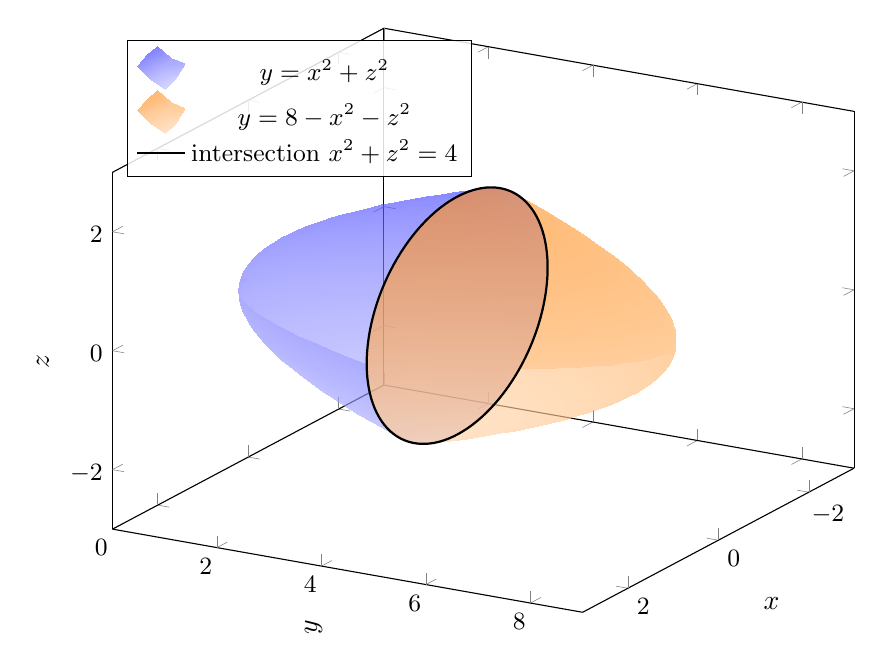
\begin{tikzpicture}
\begin{axis}[
    view={120}{25},
    axis lines=box,
    xlabel=$x$, ylabel=$y$, zlabel=$z$,
    xmin=-3, xmax=3,
    ymin=0, ymax=9,
    zmin=-3, zmax=3,
    samples=25, samples y=50,
    domain=0:2, y domain=0:360,
    width=11cm, height=9cm,
    tick label style={font=\small},
    legend style={font=\small, at={(0.02,0.98)}, anchor=north west, fill=white, fill opacity=0.85, text opacity=1}
]
\addplot3[surf, shader=interp, opacity=0.65,
    colormap={bluecmap}{color=(blue!25) color=(blue!75)},
    draw opacity=0.15]
    ({x*cos(y)}, {x^2}, {x*sin(y)});
\addlegendentry{$y=x^2+z^2$}
\addplot3[surf, shader=interp, opacity=0.65,
    colormap={orangecmap}{color=(orange!35) color=(orange!85)},
    draw opacity=0.15]
    ({x*cos(y)}, {8-x^2}, {x*sin(y)});
\addlegendentry{$y=8-x^2-z^2$}
\addplot3[thick, black, domain=0:360, samples=120, samples y=1]
    ({2*cos(x)}, {4}, {2*sin(x)});
\addlegendentry{intersection $x^2+z^2=4$}
\end{axis}
\end{tikzpicture}
\end{document}